%--
%-- Modelo de Objetivos
%--
\clearpage
\subsection{Modelo de Objetivos}

\subsubsection{Diagrama de Objetivos}
\fixme[Insertar el diagrama (no entra en una página)]

\newpage
\subsubsection{Objetivo blando: Registro del cliente}
\begin{figure}[H]
  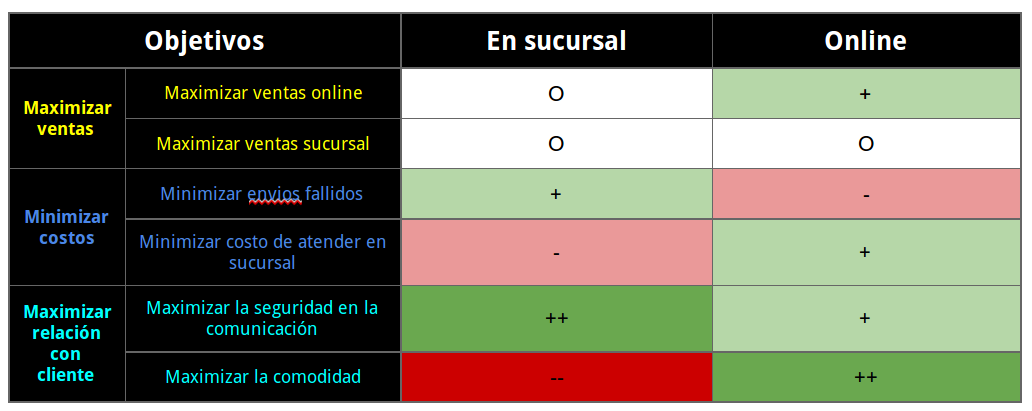
\includegraphics[width=\linewidth]{images/objetivo-blando-registro-cliente.png}
\end{figure}

\paragraph{Ventas}

La opción de registro online es evidentemente más simple y accesible, lo que
ocasionaría que más clientes opten por registrarse y comprar online, sobre todo
aquellos clientes que no acostumbran a comprar normalmente en ese supermercado
(ya que esto no impactaría tanto en los clientes habituales). De lo anterior, se
deduce que la opción de registro online impactaría positivamente en el objetivo
de maximizar las ventas online.

\paragraph{Costos}

Al obligar a los clientes a registrarse presencialmente en una sucursal,
exigiendoles la documentación correspondiente (por ejemplo, dni, un impuesto,
una factura de servicio) que acredite su domicilio y su identidad, se estaría
obteniendo una verificación confiable de los mismos, lo que repercute en una
minimización de los envíos fallidos ocasionados por personas que presentan datos
falsos, o sin ser esta su intención, cometen errores al escribir los datos. El
registro online, por el contrario, aumenta la posibilidad de que sucedan esos
inconvenientes, lo que impactaría negativamente en la minimización de los envíos
fallidos.

\paragraph{Relación con cliente}

\subparagraph{Maximizar la seguridad en la comunicación:}

Al registrar los datos del cliente en la sucursal, en persona, se presume que la
transmisión de los datos del cliente es siempre más segura que si se lo hace
online. De todos modos, según lo solicitado por el CEO, la comunicación se
establecería por un canal seguro, así que el riesgo de robo de información por
medio de una escucha de red se encuentra notablemente suprimido. Desde esa
perspectiva, ambos canales de comunicación tienen un nivel de confiabilidad
similar.

Por otro lado, mediante el canal de registro online, una persona podría llegar a
realizar un registro fraudulento, suplantando la identidad de otra persona,
escudada en el anonimato que ofrece internet, mientras que presencialmente es
mucho más difícil realizar este tipo de prácticas, de lo que concluimos que, si
bien ambos canales son seguros, la vía presencial resulta bastante más
confiable.

\subparagraph{Maximizar la comodidad:}

Obligar al cliente a realizar el registro presencialmente, suponiendo además que
este deba recolectar y presentar toda la documentación pertinente, le puede
llegar a resultar molesto e incómodo. En el peor caso el cliente tendría que
juntar y fotocopiar toda la documentación exigida, dirigirse a una sucursal en
horario laboral, no necesariamente cerca de su domicilio, esperar a ser
atendido, completar algún tipo de formulario, entregar la documentación, y
esperar a que le informen de algún modo que su usuario fue dado de alta.
Mediante el registro online, en cambio, el cliente podrá ingresar al website
desde la comodidad de su casa, en cualquier horario, e ingresar sus datos.
Inmediatamente, entonces, el cliente tendría la posibilidad de realizar una
compra.

\newpage
\subsubsection{Objetivo blando: Ranking del cliente}
\begin{figure}[H]
  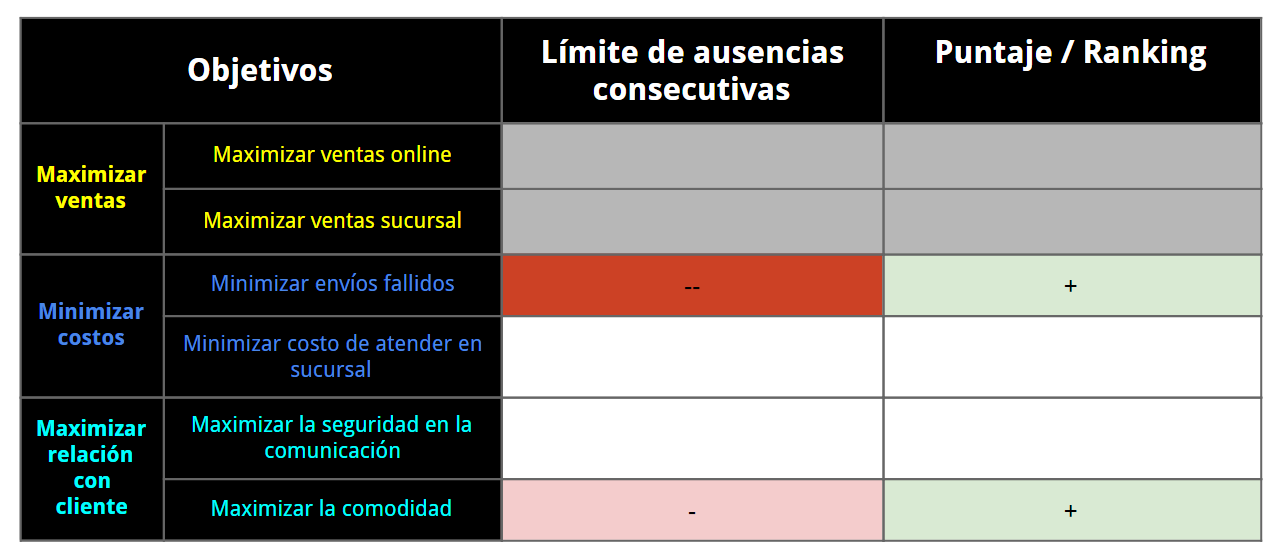
\includegraphics[width=\linewidth]{images/objetivo-blando-ranking-cliente.png}
\end{figure}

\fixme[Agregar completar tabla y agregar texto justificando los puntajes]